\documentclass[11pt,a4paper]{article}
\usepackage[margin=2.2cm]{geometry}
\usepackage{times}
\usepackage{booktabs}
\usepackage{tikz}
\usetikzlibrary{positioning,arrows.meta}
\setlength{\parindent}{0pt}
\setlength{\parskip}{6pt}

\title{Virtual Switch\\[2pt]\large Operating Systems, Fall 2026}
\author{Umair Abbas \quad (bsai24077)}
\date{}

\begin{document}
\maketitle
\vspace{-1.5em}

\section{Overview}

The switch is a multithreaded TCP server in C. Each host connects to one
port and sends frames in the fixed 17-byte header format. The switch learns
which MAC is on which port, forwards frames only where they need to go, and
floods broadcasts and unknown destinations inside the frame's VLAN.
An admin tool, \texttt{swctl}, talks to the switch over a UNIX domain socket
and reads live counters from shared memory.

\textbf{Completed:} all of Tier 1 (items 1--5), all of Tier 2 (items 6--13), and all
three Tier 3 items: two switches over pipes, the supervisor, and the benchmark.

The switch is clean under ThreadSanitizer and valgrind (0 errors, 0 bytes in
use at exit) while running my tests: forwarding, partial frames, a frozen
host, a full switch, port security, VLANs, mirroring, rate limiting, QoS, and
about 180 admin commands while 10,000 frames were flowing.

\section{Threads}

\begin{center}
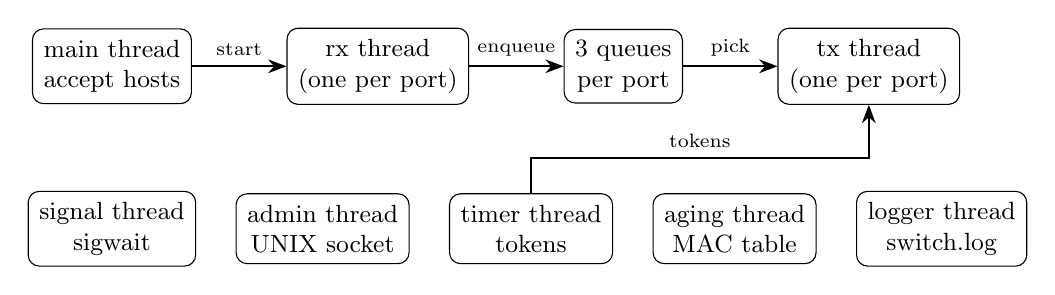
\begin{tikzpicture}[
  box/.style={draw, rounded corners, align=center, font=\small, minimum height=8mm, inner sep=4pt},
  arr/.style={-{Stealth}, thick}]
\node[box] (main) {main thread\\accept hosts};
\node[box, right=1.2cm of main] (rx) {rx thread\\(one per port)};
\node[box, right=1.2cm of rx] (q) {3 queues\\per port};
\node[box, right=1.2cm of q] (tx) {tx thread\\(one per port)};
\node[box, below=1.1cm of main] (sig) {signal thread\\sigwait};
\node[box, right=0.5cm of sig] (admin) {admin thread\\UNIX socket};
\node[box, right=0.5cm of admin] (timer) {timer thread\\tokens};
\node[box, right=0.5cm of timer] (age) {aging thread\\MAC table};
\node[box, right=0.5cm of age] (log) {logger thread\\switch.log};
\draw[arr] (main) -- node[above, font=\scriptsize]{start} (rx);
\draw[arr] (rx) -- node[above, font=\scriptsize]{enqueue} (q);
\draw[arr] (q) -- node[above, font=\scriptsize]{pick} (tx);
\draw[arr] (timer.north) -- ++(0,0.45) -| node[pos=0.25, above, font=\scriptsize]{tokens} (tx.south);
\end{tikzpicture}
\end{center}

\begin{tabular}{@{}lp{12.3cm}@{}}
\toprule
Thread & What it does \\
\midrule
main & Accepts hosts. Waits on the free-port semaphore with \texttt{sem\_timedwait};
       on timeout it sends ``switch full''. Starts the rx and tx threads of a port. \\
rx (per port) & Reads frames (from a socket, or from a pipe for the trunk link), learns the source MAC, checks port security,
       sends a mirror copy, and puts the frame on the output queues. Never blocks on a full queue. \\
tx (per port) & Picks the next frame with weighted round robin, waits for a token,
       writes it to the host, and frees the frame when it is the last user. \\
timer & Every 100 ms adds tokens to each port's bucket and wakes the tx threads. \\
aging & Every 5 s removes MACs older than the aging time. \\
admin & Accepts \texttt{swctl} connections and runs one command each. \\
signal & The only thread that gets signals (\texttt{sigwait}).
       SIGINT: clean shutdown, SIGHUP: reload config, SIGUSR1: dump MAC table. \\
logger & Takes messages from the log queue and writes them with timestamps. \\
\bottomrule
\end{tabular}

All signals are blocked in \texttt{main()} before any thread is created, so every
thread inherits the mask. SIGPIPE is ignored; a failed write just marks the host dead.

\section{Locks}

\begin{tabular}{@{}lp{11.2cm}@{}}
\toprule
Lock & What it protects \\
\midrule
\texttt{ports\_lock} & Port state (free, used, down), who must join the rx thread, the ``shut down by admin'' flag. \\
\texttt{ports[i].lock} & The port's 3 queues, round-robin state, tokens, rate, VLAN, trunk flag, mirror target, socket fd.
                         Two condition variables use it: \texttt{not\_empty} and \texttt{can\_send}. \\
bucket locks (16) & One per hash bucket of the MAC table (striped locking). \\
\texttt{count\_lock} & Number of MAC entries and the list of free entries. \\
frame lock & The reference count of one frame. \\
\texttt{cfg\_lock} & Global settings: aging time, port security limit, wait time. \\
\texttt{stop\_lock} & The stop flag. \texttt{stop\_cond} wakes the timer and aging threads. \\
stats lock & Counters in shared memory. Process-shared, so \texttt{swctl} can use it too. \\
logger lock & The log message queue. \\
semaphore & Number of free ports (counting semaphore, not a lock). \\
\bottomrule
\end{tabular}

A broadcast frame is not copied. It goes into every queue with its reference
count raised by one each time. Each tx thread lowers the count after sending, and
the one that brings it to zero frees the frame.

\section{Lock order}

When a thread holds more than one lock, it always takes them in this order:

\begin{enumerate}
\setlength{\itemsep}{0pt}
\item \texttt{ports\_lock}
\item \texttt{ports[i].lock}, in increasing port number when several are held
\item MAC table bucket locks in increasing bucket number, then \texttt{count\_lock}
\item frame lock
\end{enumerate}

\texttt{cfg\_lock}, \texttt{stop\_lock}, the stats lock and the logger lock are
\emph{leaf} locks: nothing else is taken while one of them is held.

Commands that touch several ports (\texttt{trunk}, SIGHUP reload) lock all
ports from 0 to $N-1$ and unlock in reverse. \texttt{clear mac} locks buckets
0 to 15 the same way. The rx thread never holds its own port lock while putting a
frame on another port, so two ports sending to each other cannot deadlock.

Shutting a port down: the admin thread sets the ``down'' flag under
\texttt{ports\_lock}, shuts the socket, releases the lock, then joins the rx thread.
The rx thread closes the port (wakes and joins the tx thread, which drops what is
left in the queues and frees it) and marks the port down. Only one thread can ever join a
given rx thread, because the ``must join'' flag is claimed under \texttt{ports\_lock}.

\section{A real bug}

\textbf{Bug.} For the supervisor, the MAC table lives in shared memory so it
survives a crash. My test learned two MACs, killed the switch with SIGKILL, and
checked \texttt{swctl show mac} after the supervisor restarted it. The test failed:
the table was empty. But the log said
\emph{``MAC table restored from shared memory: 2 entries''}.

\textbf{How I found it.} So the restore worked and something removed the entries
right after. I looked at everything that runs between the restore and the first
command. \texttt{apply\_config()} compares each port's VLAN with the config file
and, if it changed, flushes that port's MACs (needed when an admin moves a port to
another VLAN). At startup the ports came from \texttt{calloc}, so their VLAN was 0,
the config said 1, every port looked ``changed'', and every MAC was flushed.

\textbf{Fix.} Each port now starts with its VLAN and trunk flag taken from the config,
so the first \texttt{apply\_config()} sees no change. After the fix the table
survives both SIGKILL and SIGSEGV, and the earlier tests still pass.

\section{Tier 3}

\textbf{Two switches.} \texttt{./twoswitch} makes two pipes and forks two switches
(as in \texttt{two\_way.c}, Lab 05). Each child keeps only its read end and its write
end, so the other side sees EOF when it exits. Each switch uses its last port as the
trunk over these pipes. A pipe cannot be \texttt{shutdown()} like a socket, so the
trunk rx thread waits with \texttt{poll()} on the pipe and on a small ``wake'' pipe;
writing one byte to the wake pipe stops it. Hosts on A reach hosts on B in the same
VLAN, and each switch learns the other's hosts on its trunk port.

\textbf{Supervisor.} \texttt{./supervisor} forks the switch and waits with
\texttt{waitpid}. If the switch dies from a signal it is started again with
\texttt{-r}. The MAC table is one shared memory block: entries are linked by array
index instead of pointer, and the locks are process-shared. On restore the old
process may have died in the middle of a change, so the switch does not trust the
chains: it makes the locks again and rebuilds the chains and free list from each
entry's ``used'' flag. A clean exit (status 0) stops the supervisor too.

\textbf{Benchmark.} See the separate one-page benchmark report (\texttt{benchmark.pdf}).
Striped locks scale with threads; a global lock and a read-write lock get slower.

\end{document}
